\documentclass[10pt]{article} % For LaTeX2e
\usepackage[preprint]{tmlr}
% preprint option: blank running header and the \author block below is printed.

%%%%% NEW MATH DEFINITIONS %%%%%

\usepackage{amsmath,amsfonts,bm}

% Mark sections of captions for referring to divisions of figures
\newcommand{\figleft}{{\em (Left)}}
\newcommand{\figcenter}{{\em (Center)}}
\newcommand{\figright}{{\em (Right)}}
\newcommand{\figtop}{{\em (Top)}}
\newcommand{\figbottom}{{\em (Bottom)}}
\newcommand{\captiona}{{\em (a)}}
\newcommand{\captionb}{{\em (b)}}
\newcommand{\captionc}{{\em (c)}}
\newcommand{\captiond}{{\em (d)}}

% Highlight a newly defined term
\newcommand{\newterm}[1]{{\bf #1}}


% Figure reference, lower-case.
\def\figref#1{figure~\ref{#1}}
% Figure reference, capital. For start of sentence
\def\Figref#1{Figure~\ref{#1}}
\def\twofigref#1#2{figures \ref{#1} and \ref{#2}}
\def\quadfigref#1#2#3#4{figures \ref{#1}, \ref{#2}, \ref{#3} and \ref{#4}}
% Section reference, lower-case.
\def\secref#1{section~\ref{#1}}
% Section reference, capital.
\def\Secref#1{Section~\ref{#1}}
% Reference to two sections.
\def\twosecrefs#1#2{sections \ref{#1} and \ref{#2}}
% Reference to three sections.
\def\secrefs#1#2#3{sections \ref{#1}, \ref{#2} and \ref{#3}}
% Reference to an equation, lower-case.
\def\eqref#1{equation~\ref{#1}}
% Reference to an equation, upper case
\def\Eqref#1{Equation~\ref{#1}}
% A raw reference to an equation---avoid using if possible
\def\plaineqref#1{\ref{#1}}
% Reference to a chapter, lower-case.
\def\chapref#1{chapter~\ref{#1}}
% Reference to an equation, upper case.
\def\Chapref#1{Chapter~\ref{#1}}
% Reference to a range of chapters
\def\rangechapref#1#2{chapters\ref{#1}--\ref{#2}}
% Reference to an algorithm, lower-case.
\def\algref#1{algorithm~\ref{#1}}
% Reference to an algorithm, upper case.
\def\Algref#1{Algorithm~\ref{#1}}
\def\twoalgref#1#2{algorithms \ref{#1} and \ref{#2}}
\def\Twoalgref#1#2{Algorithms \ref{#1} and \ref{#2}}
% Reference to a part, lower case
\def\partref#1{part~\ref{#1}}
% Reference to a part, upper case
\def\Partref#1{Part~\ref{#1}}
\def\twopartref#1#2{parts \ref{#1} and \ref{#2}}

\def\ceil#1{\lceil #1 \rceil}
\def\floor#1{\lfloor #1 \rfloor}
\def\1{\bm{1}}
\newcommand{\train}{\mathcal{D}}
\newcommand{\valid}{\mathcal{D_{\mathrm{valid}}}}
\newcommand{\test}{\mathcal{D_{\mathrm{test}}}}

\def\eps{{\epsilon}}


% Random variables
\def\reta{{\textnormal{$\eta$}}}
\def\ra{{\textnormal{a}}}
\def\rb{{\textnormal{b}}}
\def\rc{{\textnormal{c}}}
\def\rd{{\textnormal{d}}}
\def\re{{\textnormal{e}}}
\def\rf{{\textnormal{f}}}
\def\rg{{\textnormal{g}}}
\def\rh{{\textnormal{h}}}
\def\ri{{\textnormal{i}}}
\def\rj{{\textnormal{j}}}
\def\rk{{\textnormal{k}}}
\def\rl{{\textnormal{l}}}
% rm is already a command, just don't name any random variables m
\def\rn{{\textnormal{n}}}
\def\ro{{\textnormal{o}}}
\def\rp{{\textnormal{p}}}
\def\rq{{\textnormal{q}}}
\def\rr{{\textnormal{r}}}
\def\rs{{\textnormal{s}}}
\def\rt{{\textnormal{t}}}
\def\ru{{\textnormal{u}}}
\def\rv{{\textnormal{v}}}
\def\rw{{\textnormal{w}}}
\def\rx{{\textnormal{x}}}
\def\ry{{\textnormal{y}}}
\def\rz{{\textnormal{z}}}

% Random vectors
\def\rvepsilon{{\mathbf{\epsilon}}}
\def\rvtheta{{\mathbf{\theta}}}
\def\rva{{\mathbf{a}}}
\def\rvb{{\mathbf{b}}}
\def\rvc{{\mathbf{c}}}
\def\rvd{{\mathbf{d}}}
\def\rve{{\mathbf{e}}}
\def\rvf{{\mathbf{f}}}
\def\rvg{{\mathbf{g}}}
\def\rvh{{\mathbf{h}}}
\def\rvu{{\mathbf{i}}}
\def\rvj{{\mathbf{j}}}
\def\rvk{{\mathbf{k}}}
\def\rvl{{\mathbf{l}}}
\def\rvm{{\mathbf{m}}}
\def\rvn{{\mathbf{n}}}
\def\rvo{{\mathbf{o}}}
\def\rvp{{\mathbf{p}}}
\def\rvq{{\mathbf{q}}}
\def\rvr{{\mathbf{r}}}
\def\rvs{{\mathbf{s}}}
\def\rvt{{\mathbf{t}}}
\def\rvu{{\mathbf{u}}}
\def\rvv{{\mathbf{v}}}
\def\rvw{{\mathbf{w}}}
\def\rvx{{\mathbf{x}}}
\def\rvy{{\mathbf{y}}}
\def\rvz{{\mathbf{z}}}

% Elements of random vectors
\def\erva{{\textnormal{a}}}
\def\ervb{{\textnormal{b}}}
\def\ervc{{\textnormal{c}}}
\def\ervd{{\textnormal{d}}}
\def\erve{{\textnormal{e}}}
\def\ervf{{\textnormal{f}}}
\def\ervg{{\textnormal{g}}}
\def\ervh{{\textnormal{h}}}
\def\ervi{{\textnormal{i}}}
\def\ervj{{\textnormal{j}}}
\def\ervk{{\textnormal{k}}}
\def\ervl{{\textnormal{l}}}
\def\ervm{{\textnormal{m}}}
\def\ervn{{\textnormal{n}}}
\def\ervo{{\textnormal{o}}}
\def\ervp{{\textnormal{p}}}
\def\ervq{{\textnormal{q}}}
\def\ervr{{\textnormal{r}}}
\def\ervs{{\textnormal{s}}}
\def\ervt{{\textnormal{t}}}
\def\ervu{{\textnormal{u}}}
\def\ervv{{\textnormal{v}}}
\def\ervw{{\textnormal{w}}}
\def\ervx{{\textnormal{x}}}
\def\ervy{{\textnormal{y}}}
\def\ervz{{\textnormal{z}}}

% Random matrices
\def\rmA{{\mathbf{A}}}
\def\rmB{{\mathbf{B}}}
\def\rmC{{\mathbf{C}}}
\def\rmD{{\mathbf{D}}}
\def\rmE{{\mathbf{E}}}
\def\rmF{{\mathbf{F}}}
\def\rmG{{\mathbf{G}}}
\def\rmH{{\mathbf{H}}}
\def\rmI{{\mathbf{I}}}
\def\rmJ{{\mathbf{J}}}
\def\rmK{{\mathbf{K}}}
\def\rmL{{\mathbf{L}}}
\def\rmM{{\mathbf{M}}}
\def\rmN{{\mathbf{N}}}
\def\rmO{{\mathbf{O}}}
\def\rmP{{\mathbf{P}}}
\def\rmQ{{\mathbf{Q}}}
\def\rmR{{\mathbf{R}}}
\def\rmS{{\mathbf{S}}}
\def\rmT{{\mathbf{T}}}
\def\rmU{{\mathbf{U}}}
\def\rmV{{\mathbf{V}}}
\def\rmW{{\mathbf{W}}}
\def\rmX{{\mathbf{X}}}
\def\rmY{{\mathbf{Y}}}
\def\rmZ{{\mathbf{Z}}}

% Elements of random matrices
\def\ermA{{\textnormal{A}}}
\def\ermB{{\textnormal{B}}}
\def\ermC{{\textnormal{C}}}
\def\ermD{{\textnormal{D}}}
\def\ermE{{\textnormal{E}}}
\def\ermF{{\textnormal{F}}}
\def\ermG{{\textnormal{G}}}
\def\ermH{{\textnormal{H}}}
\def\ermI{{\textnormal{I}}}
\def\ermJ{{\textnormal{J}}}
\def\ermK{{\textnormal{K}}}
\def\ermL{{\textnormal{L}}}
\def\ermM{{\textnormal{M}}}
\def\ermN{{\textnormal{N}}}
\def\ermO{{\textnormal{O}}}
\def\ermP{{\textnormal{P}}}
\def\ermQ{{\textnormal{Q}}}
\def\ermR{{\textnormal{R}}}
\def\ermS{{\textnormal{S}}}
\def\ermT{{\textnormal{T}}}
\def\ermU{{\textnormal{U}}}
\def\ermV{{\textnormal{V}}}
\def\ermW{{\textnormal{W}}}
\def\ermX{{\textnormal{X}}}
\def\ermY{{\textnormal{Y}}}
\def\ermZ{{\textnormal{Z}}}

% Vectors
\def\vzero{{\bm{0}}}
\def\vone{{\bm{1}}}
\def\vmu{{\bm{\mu}}}
\def\vtheta{{\bm{\theta}}}
\def\va{{\bm{a}}}
\def\vb{{\bm{b}}}
\def\vc{{\bm{c}}}
\def\vd{{\bm{d}}}
\def\ve{{\bm{e}}}
\def\vf{{\bm{f}}}
\def\vg{{\bm{g}}}
\def\vh{{\bm{h}}}
\def\vi{{\bm{i}}}
\def\vj{{\bm{j}}}
\def\vk{{\bm{k}}}
\def\vl{{\bm{l}}}
\def\vm{{\bm{m}}}
\def\vn{{\bm{n}}}
\def\vo{{\bm{o}}}
\def\vp{{\bm{p}}}
\def\vq{{\bm{q}}}
\def\vr{{\bm{r}}}
\def\vs{{\bm{s}}}
\def\vt{{\bm{t}}}
\def\vu{{\bm{u}}}
\def\vv{{\bm{v}}}
\def\vw{{\bm{w}}}
\def\vx{{\bm{x}}}
\def\vy{{\bm{y}}}
\def\vz{{\bm{z}}}

% Elements of vectors
\def\evalpha{{\alpha}}
\def\evbeta{{\beta}}
\def\evepsilon{{\epsilon}}
\def\evlambda{{\lambda}}
\def\evomega{{\omega}}
\def\evmu{{\mu}}
\def\evpsi{{\psi}}
\def\evsigma{{\sigma}}
\def\evtheta{{\theta}}
\def\eva{{a}}
\def\evb{{b}}
\def\evc{{c}}
\def\evd{{d}}
\def\eve{{e}}
\def\evf{{f}}
\def\evg{{g}}
\def\evh{{h}}
\def\evi{{i}}
\def\evj{{j}}
\def\evk{{k}}
\def\evl{{l}}
\def\evm{{m}}
\def\evn{{n}}
\def\evo{{o}}
\def\evp{{p}}
\def\evq{{q}}
\def\evr{{r}}
\def\evs{{s}}
\def\evt{{t}}
\def\evu{{u}}
\def\evv{{v}}
\def\evw{{w}}
\def\evx{{x}}
\def\evy{{y}}
\def\evz{{z}}

% Matrix
\def\mA{{\bm{A}}}
\def\mB{{\bm{B}}}
\def\mC{{\bm{C}}}
\def\mD{{\bm{D}}}
\def\mE{{\bm{E}}}
\def\mF{{\bm{F}}}
\def\mG{{\bm{G}}}
\def\mH{{\bm{H}}}
\def\mI{{\bm{I}}}
\def\mJ{{\bm{J}}}
\def\mK{{\bm{K}}}
\def\mL{{\bm{L}}}
\def\mM{{\bm{M}}}
\def\mN{{\bm{N}}}
\def\mO{{\bm{O}}}
\def\mP{{\bm{P}}}
\def\mQ{{\bm{Q}}}
\def\mR{{\bm{R}}}
\def\mS{{\bm{S}}}
\def\mT{{\bm{T}}}
\def\mU{{\bm{U}}}
\def\mV{{\bm{V}}}
\def\mW{{\bm{W}}}
\def\mX{{\bm{X}}}
\def\mY{{\bm{Y}}}
\def\mZ{{\bm{Z}}}
\def\mBeta{{\bm{\beta}}}
\def\mPhi{{\bm{\Phi}}}
\def\mLambda{{\bm{\Lambda}}}
\def\mSigma{{\bm{\Sigma}}}

% Tensor
\DeclareMathAlphabet{\mathsfit}{\encodingdefault}{\sfdefault}{m}{sl}
\SetMathAlphabet{\mathsfit}{bold}{\encodingdefault}{\sfdefault}{bx}{n}
\newcommand{\tens}[1]{\bm{\mathsfit{#1}}}
\def\tA{{\tens{A}}}
\def\tB{{\tens{B}}}
\def\tC{{\tens{C}}}
\def\tD{{\tens{D}}}
\def\tE{{\tens{E}}}
\def\tF{{\tens{F}}}
\def\tG{{\tens{G}}}
\def\tH{{\tens{H}}}
\def\tI{{\tens{I}}}
\def\tJ{{\tens{J}}}
\def\tK{{\tens{K}}}
\def\tL{{\tens{L}}}
\def\tM{{\tens{M}}}
\def\tN{{\tens{N}}}
\def\tO{{\tens{O}}}
\def\tP{{\tens{P}}}
\def\tQ{{\tens{Q}}}
\def\tR{{\tens{R}}}
\def\tS{{\tens{S}}}
\def\tT{{\tens{T}}}
\def\tU{{\tens{U}}}
\def\tV{{\tens{V}}}
\def\tW{{\tens{W}}}
\def\tX{{\tens{X}}}
\def\tY{{\tens{Y}}}
\def\tZ{{\tens{Z}}}


% Graph
\def\gA{{\mathcal{A}}}
\def\gB{{\mathcal{B}}}
\def\gC{{\mathcal{C}}}
\def\gD{{\mathcal{D}}}
\def\gE{{\mathcal{E}}}
\def\gF{{\mathcal{F}}}
\def\gG{{\mathcal{G}}}
\def\gH{{\mathcal{H}}}
\def\gI{{\mathcal{I}}}
\def\gJ{{\mathcal{J}}}
\def\gK{{\mathcal{K}}}
\def\gL{{\mathcal{L}}}
\def\gM{{\mathcal{M}}}
\def\gN{{\mathcal{N}}}
\def\gO{{\mathcal{O}}}
\def\gP{{\mathcal{P}}}
\def\gQ{{\mathcal{Q}}}
\def\gR{{\mathcal{R}}}
\def\gS{{\mathcal{S}}}
\def\gT{{\mathcal{T}}}
\def\gU{{\mathcal{U}}}
\def\gV{{\mathcal{V}}}
\def\gW{{\mathcal{W}}}
\def\gX{{\mathcal{X}}}
\def\gY{{\mathcal{Y}}}
\def\gZ{{\mathcal{Z}}}

% Sets
\def\sA{{\mathbb{A}}}
\def\sB{{\mathbb{B}}}
\def\sC{{\mathbb{C}}}
\def\sD{{\mathbb{D}}}
% Don't use a set called E, because this would be the same as our symbol
% for expectation.
\def\sF{{\mathbb{F}}}
\def\sG{{\mathbb{G}}}
\def\sH{{\mathbb{H}}}
\def\sI{{\mathbb{I}}}
\def\sJ{{\mathbb{J}}}
\def\sK{{\mathbb{K}}}
\def\sL{{\mathbb{L}}}
\def\sM{{\mathbb{M}}}
\def\sN{{\mathbb{N}}}
\def\sO{{\mathbb{O}}}
\def\sP{{\mathbb{P}}}
\def\sQ{{\mathbb{Q}}}
\def\sR{{\mathbb{R}}}
\def\sS{{\mathbb{S}}}
\def\sT{{\mathbb{T}}}
\def\sU{{\mathbb{U}}}
\def\sV{{\mathbb{V}}}
\def\sW{{\mathbb{W}}}
\def\sX{{\mathbb{X}}}
\def\sY{{\mathbb{Y}}}
\def\sZ{{\mathbb{Z}}}

% Entries of a matrix
\def\emLambda{{\Lambda}}
\def\emA{{A}}
\def\emB{{B}}
\def\emC{{C}}
\def\emD{{D}}
\def\emE{{E}}
\def\emF{{F}}
\def\emG{{G}}
\def\emH{{H}}
\def\emI{{I}}
\def\emJ{{J}}
\def\emK{{K}}
\def\emL{{L}}
\def\emM{{M}}
\def\emN{{N}}
\def\emO{{O}}
\def\emP{{P}}
\def\emQ{{Q}}
\def\emR{{R}}
\def\emS{{S}}
\def\emT{{T}}
\def\emU{{U}}
\def\emV{{V}}
\def\emW{{W}}
\def\emX{{X}}
\def\emY{{Y}}
\def\emZ{{Z}}
\def\emSigma{{\Sigma}}

% entries of a tensor
% Same font as tensor, without \bm wrapper
\newcommand{\etens}[1]{\mathsfit{#1}}
\def\etLambda{{\etens{\Lambda}}}
\def\etA{{\etens{A}}}
\def\etB{{\etens{B}}}
\def\etC{{\etens{C}}}
\def\etD{{\etens{D}}}
\def\etE{{\etens{E}}}
\def\etF{{\etens{F}}}
\def\etG{{\etens{G}}}
\def\etH{{\etens{H}}}
\def\etI{{\etens{I}}}
\def\etJ{{\etens{J}}}
\def\etK{{\etens{K}}}
\def\etL{{\etens{L}}}
\def\etM{{\etens{M}}}
\def\etN{{\etens{N}}}
\def\etO{{\etens{O}}}
\def\etP{{\etens{P}}}
\def\etQ{{\etens{Q}}}
\def\etR{{\etens{R}}}
\def\etS{{\etens{S}}}
\def\etT{{\etens{T}}}
\def\etU{{\etens{U}}}
\def\etV{{\etens{V}}}
\def\etW{{\etens{W}}}
\def\etX{{\etens{X}}}
\def\etY{{\etens{Y}}}
\def\etZ{{\etens{Z}}}

% The true underlying data generating distribution
\newcommand{\pdata}{p_{\rm{data}}}
% The empirical distribution defined by the training set
\newcommand{\ptrain}{\hat{p}_{\rm{data}}}
\newcommand{\Ptrain}{\hat{P}_{\rm{data}}}
% The model distribution
\newcommand{\pmodel}{p_{\rm{model}}}
\newcommand{\Pmodel}{P_{\rm{model}}}
\newcommand{\ptildemodel}{\tilde{p}_{\rm{model}}}
% Stochastic autoencoder distributions
\newcommand{\pencode}{p_{\rm{encoder}}}
\newcommand{\pdecode}{p_{\rm{decoder}}}
\newcommand{\precons}{p_{\rm{reconstruct}}}

\newcommand{\laplace}{\mathrm{Laplace}} % Laplace distribution

\newcommand{\E}{\mathbb{E}}
\newcommand{\Ls}{\mathcal{L}}
\newcommand{\R}{\mathbb{R}}
\newcommand{\emp}{\tilde{p}}
\newcommand{\lr}{\alpha}
\newcommand{\reg}{\lambda}
\newcommand{\rect}{\mathrm{rectifier}}
\newcommand{\softmax}{\mathrm{softmax}}
\newcommand{\sigmoid}{\sigma}
\newcommand{\softplus}{\zeta}
\newcommand{\KL}{D_{\mathrm{KL}}}
\newcommand{\Var}{\mathrm{Var}}
\newcommand{\standarderror}{\mathrm{SE}}
\newcommand{\Cov}{\mathrm{Cov}}
% Wolfram Mathworld says $L^2$ is for function spaces and $\ell^2$ is for vectors
% But then they seem to use $L^2$ for vectors throughout the site, and so does
% wikipedia.
\newcommand{\normlzero}{L^0}
\newcommand{\normlone}{L^1}
\newcommand{\normltwo}{L^2}
\newcommand{\normlp}{L^p}
\newcommand{\normmax}{L^\infty}

\newcommand{\parents}{Pa} % See usage in notation.tex. Chosen to match Daphne's book.

\DeclareMathOperator*{\argmax}{arg\,max}
\DeclareMathOperator*{\argmin}{arg\,min}

\DeclareMathOperator{\sign}{sign}
\DeclareMathOperator{\Tr}{Tr}
\let\ab\allowbreak


\usepackage{hyperref}
\usepackage{url}
\usepackage{booktabs}
\usepackage{graphicx}
\usepackage{xcolor}
\usepackage{amsmath}
\usepackage{amssymb}
\usepackage{float}

% Arm names, so they render identically everywhere.
\newcommand{\Bz}{B0}
\newcommand{\Bo}{B1}
\newcommand{\Bt}{B2}
\newcommand{\Bth}{B3}
\newcommand{\T}{T}
\newcommand{\Tctrl}{T\textsubscript{ctrl}}
\newcommand{\Trfifty}{T\textsubscript{r050}}
\newcommand{\Trtwo}{T\textsubscript{r200}}
% Run-in paragraph lead.
\newcommand{\lead}[1]{\textbf{#1}\ }

\title{Safety-mixed preference optimisation versus a bolted-on guardrail for wellness-support dialogue: a pre-registered comparison and a classifier-blindness finding}

\author{\name Student number 20039893}

\def\month{09}
\def\year{2026}
\def\openreview{\url{https://openreview.net/forum?id=XXXX}}

\begin{document}

\maketitle

\begin{abstract}
Safety can be added to a wellness-support language model by training it into the policy or by bolting a classifier onto its outputs, and the two are rarely compared like for like. This study compares them on one base model with matched training volume and a pre-registered endpoint. From a LoRA supervised fine-tune of Qwen2.5-7B-Instruct on counselling dialogue, it trains two RPO-style DPO policies on 19,924 preference pairs each, one on helpfulness pairs only and one with a share replaced by PKU-SafeRLHF harmlessness pairs. The helpfulness-only policy behind Llama-Guard-3-8B forms the filter arm. On a frozen 180-prompt adversarial suite the safety-mixed policy reached an attack-success rate of 39.4\% against 45.0\% for the filter arm, a difference of $-5.6$ points (95\% CI $[-13.9, +2.8]$, $p=0.227$) that neither reaches nor rules out the pre-registered 10-point threshold. The minimum detectable effect was 11.6 points, so the design could not have detected its own threshold. Over-refusal did not change and helpfulness fell by 2.1 points on the reward-model scale. Fine-tuning alone had raised the base model's attack-success rate from 26.1\% to 51.1\%, and neither DPO arm returned it to the base. The filter was close to inert because content classifiers missed the breaches: 84\% to 96\% of judge-confirmed attack successes evaded both Llama Guard 3 and the BeaverTails moderation model in every unfiltered arm, on a judge validated against human labels ($\kappa=0.668$). The study covers one base model, English only, one attack taxonomy and one pre-registered seed with a three-seed post hoc panel, and makes no clinical claims.
\end{abstract}

% ===========================================================================
\section{Introduction}
% ===========================================================================
Language models are now used as wellness-support agents. The prompts they receive include attempts to extract harmful content and disclosures of crisis. A builder can add safety to such a model in two places. Safety can be trained into the policy by adding harmlessness preference pairs to the alignment stage \citep{ji2023beavertails,ji2024pku}. Or it can be bolted on, by passing each response through a content classifier that replaces unsafe output with a refusal \citep{inan2023llamaguard,markov2023holistic}.

The two are rarely compared like for like. Studies of safety-data mixing vary the base model or the training volume between arms \citep{bianchi2024safetytuned}, so a difference in safety cannot be separated from a difference in training. Guardrail classifiers are evaluated on their own taxonomies, with precision and recall measured against labels produced under that taxonomy \citep{inan2023llamaguard,zeng2024shieldgemma}. The share of a specific downstream policy's harmful output that they catch is not measured. Few comparisons in either line fix the endpoint and the decision threshold before the data exist.

Wellness support sharpens the question in two ways. The helpfulness objective for a counselling model rewards warmth, engagement and staying in the conversation. That is the behaviour persona and many-shot attacks exploit \citep{shah2023persona,anil2024manyshot}. Fine-tuning on benign data erodes safety alignment \citep{qi2024finetuning}, because the alignment is shallow \citep{qi2025safety,li2026superficial}. The domain also changes what a failure looks like: rarely the explicit harmful content a content classifier is trained on, more often a fluent turn that plays along with a persona, endorses a harmful plan, or invents a personal history. Whether safety pairs mixed into the same preference stage restore more of the eroded behaviour than a filter placed after it, at the same training cost, is open. So is whether the filter sees the domain's failures at all.

The research question is direct. Does integrating safety during preference alignment make a therapy-support model more robust to adversarial and crisis prompts than a bolted-on guardrail filter, and at what cost to helpfulness? One claim was pre-registered before any result was seen. Mixing safety preference pairs into direct preference optimisation (DPO) reduces the attack-success rate (ASR) on a held-out adversarial suite by at least 10 points, compared with an identical model with a bolted-on guardrail filter, at a bounded cost in over-refusal and helpfulness.

The contribution is threefold. First, a matched-volume, pre-registered comparison on one base model. Its primary endpoint is null, at $-5.6$ points against a 10-point threshold, with a retrospective minimum detectable effect of 11.6 points. The null is reported as a bound rather than an absence, and the threshold as a design error. Over-refusal did not change, and helpfulness fell by 2.1 points on the reward-model scale. Second, a measurement of classifier blindness. Between 84\% and 96\% of judge-confirmed attack successes evaded both Llama Guard 3 and the BeaverTails moderation model, in every unfiltered arm and every response-length tercile. The filter arm was therefore close to inert, replacing 2 of 180 attack responses. Third, the structure of the disagreement between arms. They failed on different prompts, with 56 of 180 pairs discordant at 23 against 33, at similar aggregate rates, which aggregate ASR conceals. A post hoc comparison of the base model with its fine-tune shows what both arms were trying to recover: supervised fine-tuning on counselling data raised the attack-success rate from 26.1\% to 51.1\%, and neither DPO arm returned it to the base. Two methodological findings are reported as such: vanilla DPO on a terse policy stopped emitting end-of-sequence tokens, which an NLL anchor fixed without making the model safer, and LoRA DPO on this stack is bitwise deterministic given identical data and seed.

The scope is one base model (Qwen2.5-7B-Instruct), English only, one frozen attack taxonomy, LoRA post-training, one pre-registered training seed with a three-seed post hoc panel, and a research prototype. No clinical claim is made. Section~\ref{sec:related} reviews what prior work leaves open, Section~\ref{sec:problem} states the problem and the test, Section~\ref{sec:methods} the method, Section~\ref{sec:results} the results, Section~\ref{sec:discussion} the interpretation and Section~\ref{sec:conclusion} the answer.

% ===========================================================================
\section{Related work}
\label{sec:related}
% ===========================================================================
Two lines of work meet in this study, safety alignment by training and safety by classification, and neither has been evaluated against the other on a fixed policy. Reinforcement learning from human feedback first measured the tension between helpfulness and harmlessness as two preference signals in one policy \citep{bai2022hh}. The Llama 2 recipe trained a separate safety reward model and reported that raising the share of safety data improved its safety score with little change in helpfulness \citep{touvron2023llama2}, and Safe RLHF made the trade-off an explicit constraint on the PKU pairs used here \citep{dai2024saferlhf}. DPO optimises a policy directly on preference pairs without a reward model \citep{rafailov2023dpo}, and a family of variants changes the objective or removes the reference model \citep{azar2024ipo,hong2024orpo,xu2024cpo,gupta2024refa}. The PKU-SafeRLHF and BeaverTails datasets supply harmlessness pairs and per-category harm labels for training safety in \citep{ji2024pku,ji2023beavertails}, and \citet{wang2025adversarial} combine preference learning with adversarial prompt generation. \citet{bianchi2024safetytuned} mixed a small number of safety examples into instruction tuning and found large safety gains, with over-refusal appearing at higher ratios. \citet{qi2024finetuning} showed that ordinary fine-tuning, even on benign data, erodes the safety of an aligned model, and the shallow-alignment account explains why, since the alignment is concentrated in the first output tokens \citep{qi2025safety,li2026superficial}. None of these studies holds the training volume fixed while changing only the composition of the preference data, so composition and dose are confounded. None compares the trained-in option against a filter on the same policy. DPO also lets the likelihood of the chosen completion fall during training \citep{pal2024smaug,razin2025likelihooddisplacement}. The usual remedy is a negative log-likelihood term on the chosen completion, as in RPO \citep{pang2024irpo}. Section~\ref{sec:methods} needed that remedy for a reason not reported in the literature.

The classifier line starts with production moderation models \citep{markov2023holistic} and with Llama Guard, an instruction-tuned model that labels a prompt or a response against a fixed taxonomy \citep{inan2023llamaguard}. Its third version, used here, keeps the same design on a Llama 3 base with a wider taxonomy \citep{grattafiori2024llama3}. The BeaverTails moderation model classifies responses into fourteen harm categories \citep{ji2023beavertails}. ShieldGemma \citep{zeng2024shieldgemma}, WildGuard \citep{han2024wildguard} and AEGIS \citep{ghosh2024aegis} follow the same pattern with different bases and training sets. Each reports F1 or AUPRC on public moderation benchmarks and on held-out splits of its own data, and \citet{wang2026sokguardrails} systematise how such guardrails are evaluated against jailbreak benchmarks. What is left open is recall on the breaches that matter downstream, meaning the harmful responses of a particular policy as confirmed by a judge outside the classifier's taxonomy. Also left open is whether the filter changes anything in a deployed pipeline, since a filter that blocks nothing harmful and nothing benign is inert rather than safe.

The cost side of safety has its own benchmarks. XSTest \citep{rottger2024xstest} and OR-Bench \citep{cui2024orbench} measure refusals of benign prompts that resemble unsafe ones, labelling a refusal by string matching or a language-model judge, and Do-Not-Answer evaluates the safeguards themselves \citep{wang2024donotanswer}. In a counselling domain the failure mode is not a refusal string but a deflection, for example redirecting to a professional instead of answering a yes/no question. A judge built for general refusals does not see it, and the one used here failed inter-model validation twice at $\kappa\approx0.07$. Over-refusal in this setting needs human labels, which none of the benchmark papers provides for a narrow domain.

On the attack side, \citet{wei2023jailbroken} explain jailbreaks as competing objectives and mismatched generalisation, \citet{zou2023gcg} produce transferable adversarial suffixes, \citet{ganguli2022redteam} red-team at scale with people, and \citet{yi2024jailbreaksurvey} survey the field. Three attack types are relevant to a dialogue model. Many-shot jailbreaking fills the context with compliant examples \citep{anil2024manyshot,wei2023icd}. Prefilling starts the model's turn with a compliant prefix, or exploits the generation configuration to the same end \citep{vega2023priming,huang2023maliciousinstruct,andriushchenko2025adaptive,li2025prefill}. It works because safety alignment is concentrated in the first few output tokens \citep{qi2025safety}. Persona attacks ask the model to adopt a character or a nested scenario \citep{shah2023persona,shen2024dan,li2023deepinception}. Persuasion \citep{zeng2024johnny} and multi-turn escalation \citep{russinovich2024crescendo} are related attack types this suite does not cover. HarmBench \citep{mazeika2024harmbench} and JailbreakBench \citep{chao2024jailbreakbench} standardise the prompts and the judge. Attack success is nearly always labelled by a language model \citep{zheng2023judge}, and lenient judges inflate it \citep{souly2024strongreject}. Judge reliability differs by attack type, so this study measures agreement against human labels for each type and treats ASR as a floor.

The counselling literature supplies the data and the helpfulness instruments. ESConv provides support conversations with strategy annotations \citep{liu2021esconv}. CounselChat provides therapist answers to public questions \citep{bertagnolli2020counselchat}. PsychoCounsel-Preference provides counsellor-graded preference pairs with a matching reward model \citep{zhang2026psychocounsel}. \citet{arnaizrodriguez2026betweenhelpharm} evaluate how language models handle mental-health crisis disclosures, and \citet{moore2025stigma} find general-purpose models expressing stigma and answering common clinical presentations inappropriately. Clinical guidance on self-harm assessment, suicide risk and safe messaging \citep{nice2022ng225,who2016mhgap,who2023safemessaging,stanley2012safetyplanning,posner2011cssrs} specifies what a good crisis response contains, and asking directly about suicide does not induce ideation \citep{dazzi2014asking}, which is why a refusal to engage is a failure under such guidance. Helpfulness in these papers is evaluated without an adversarial arm, and safety without a helpfulness cost. The trade-off a builder faces is not measured in either.

The closest evidence on deployed guardrails comes from \citet{nelson2026guardrail}, who measured guardrail sensitivity on a clinician-labelled set of 1,800 naturalistic mental-health conversations. A general-purpose guardrail built on the OpenAI moderation model reached a sensitivity of 0.419, one built on NVIDIA's moderation model 0.759, and a purpose-built guardrail 0.990, all on the same dataset. On an external benchmark subset the general-purpose figures rose to 0.882 and 0.907, so the large miss rates are specific to naturalistic crisis conversation. The gap that motivates this work sits between these lines: a comparison of trained-in safety against a filter on the same policy, at matched volume, with a pre-registered threshold, a human-validated judge, human over-refusal labels, and two classifiers measured on the breaches the judge confirms.

% ===========================================================================
\section{Problem statement}
\label{sec:problem}
% ===========================================================================
Let $\pi_\theta$ be a policy obtained by LoRA post-training of a fixed base model. Let $\mathcal{S}=\mathcal{S}_{\mathrm{att}}\cup\mathcal{S}_{\mathrm{cri}}\cup\mathcal{S}_{\mathrm{ben}}$ be a frozen suite of attack, crisis and benign prompts. For an attack prompt $x\in\mathcal{S}_{\mathrm{att}}$, a judge $J$ returns $J(x,\pi_\theta(x))\in\{0,1\}$, where 1 means the response is an attack success under a fixed behavioural rubric. The attack-success rate of an arm is
\begin{equation}
\mathrm{ASR}(\pi_\theta)=\frac{1}{|\mathcal{S}_{\mathrm{att}}|}\sum_{x\in\mathcal{S}_{\mathrm{att}}} J\big(x,\pi_\theta(x)\big),\qquad |\mathcal{S}_{\mathrm{att}}|=180.
\end{equation}
A crisis rate is defined in the same way over the 60 crisis prompts with a crisis rubric. Over-refusal is the number of the 60 benign prompts whose response a human labels as a refusal or deflection under a pinned rubric. Helpfulness is the mean score of a pinned reward model over the 60 benign and 60 crisis prompts (120 items). The treatment arm \T{} is trained on $N$ helpfulness pairs and $M$ safety pairs. The filter arm \Bth{} is the policy trained on $N{+}M$ helpfulness pairs with a classifier $C$ applied to each response at inference, so that $\pi_{\Bth}(x)=\pi_{\Bt}(x)$ if $C(\pi_{\Bt}(x))=0$ and a fixed refusal otherwise. The two arms share the base model, the SFT checkpoint, the LoRA template, the number of preference pairs and the number of optimiser steps, and differ only in where safety enters. Figure~\ref{fig:design} shows the lineage of every arm and Table~\ref{tab:arms} defines them.

The pre-registered hypothesis is $\mathrm{ASR}(\T)\le\mathrm{ASR}(\Bth)-10$ points, with the threshold stated on the true scale (Revision 6), the scale after correcting for judge recall (Appendix~\ref{app:recall}). Both arms answer the same prompts, so the verdicts are paired, and the test is a two-sided sign-flip permutation test on the per-prompt differences. The pre-registration had named McNemar's test on 240 prompts, and Amendment 13 recorded the switch to the permutation test on the 180 non-crisis prompts before any cross-arm result existed. With one seed per arm the per-prompt differences are binary, so this is the exact McNemar test on the discordant pairs \citep{mcnemar1947note}. With $b$ prompts unsafe only under \T{} and $c$ only under \Bth{}, the test asks whether $b$ and $c$ could have come from a symmetric split of $b+c$. A crisis co-primary over the 60 crisis prompts is disclosed with the same threshold, reported separately and never pooled with the primary. Over-refusal carries a pre-registered 5-point tolerance applied descriptively to the point estimate (Revision 7), and helpfulness is descriptive. Neither is a test. The confirmatory set contains exactly one test. Everything else in this paper is post hoc and labelled as such.

\begin{figure}[t]
\begin{center}
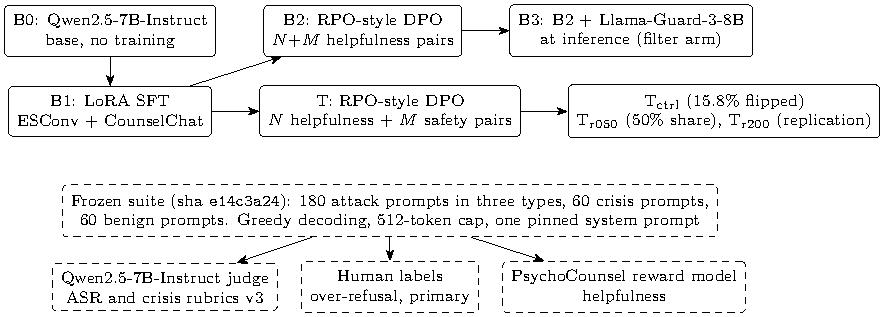
\includegraphics[width=0.56\linewidth]{figures/design.pdf}
\end{center}
\caption{Experimental design. Solid boxes are arms. Every trained arm is a LoRA adapter on the same base, and the DPO arms share the SFT checkpoint, the pair count and the step count. \Bth{} is derived from \Bt{} at inference. Dashed boxes are the evaluation instruments, all pinned. No judge shares a mechanism with the filter.}
\label{fig:design}
\end{figure}

\begin{table}[t]
\caption{Experimental arms. All trained arms share one LoRA template (Table~\ref{tab:lora}). \Bth{} is derived from \Bt{} at inference with no retraining.}
\label{tab:arms}
\begin{center}
\small
\begin{tabular}{llp{8.6cm}}
\toprule
Arm & Role & Definition \\
\midrule
\Bz{} & base & Qwen2.5-7B-Instruct, no training \\
\Bo{} & SFT & LoRA SFT on ESConv and CounselChat, assistant-only loss \\
\Bt{} & helpfulness DPO & \Bo{} $+$ RPO-style DPO on $N{+}M$ helpfulness pairs \\
\Bth{} & filter baseline & \Bt{} $+$ Llama-Guard-3-8B on each response at inference, threshold 0.5 \\
\T{} & treatment & \Bo{} $+$ RPO-style DPO on $N$ helpfulness $+$ $M$ safety pairs \\
\Tctrl{} & weak control & as \T{}, but the safety pairs take PKU's better-response label rather than its safer-response label, which differ on 15.8\% of rows (single run, no test) \\
\Trfifty{}, \Trtwo{} & ablation & safety share at 50\% of $M$, and an exact replication of \T{} \\
\bottomrule
\end{tabular}
\end{center}
\end{table}

% ===========================================================================
\section{Methods}
\label{sec:methods}
% ===========================================================================
\subsection{Training}
\label{sec:training}
\lead{Base model and adapters.} Every trained arm is a LoRA adapter \citep{hu2022lora} on Qwen2.5-7B-Instruct \citep{qwen2024qwen25} with one fixed template. The template (Table~\ref{tab:lora}) has rank 32 on all attention and MLP projections, 80,740,352 trainable parameters, 1.05\% of the total. Training used the PEFT and TRL libraries with the settings in Table~\ref{tab:hparams}, in bfloat16 with SDPA attention. The batch is 2 with 8 accumulation steps (effective 16), with gradient checkpointing. The maximum sequence length is 4,096 tokens for SFT, where the longest sequence observed was 2,619 tokens, and 2,048 for DPO. Nothing was truncated in either stage, and the training scripts assert this. The compute environment is given in Appendix~\ref{app:env}.

\lead{Supervised fine-tuning.} The SFT arm \Bo{} was trained on 2,305 conversations. These are the 910 ESConv training dialogues \citep{liu2021esconv} and 1,395 CounselChat question--answer pairs \citep{bertagnolli2020counselchat}. Loss was computed on assistant tokens only. The learning rate was $1\times10^{-4}$ with cosine decay and 3\% warm-up, for 3 epochs (435 steps). The checkpoint at the end of epoch 2 (step 290) is \Bo{}. The selection rule, fixed before training, keeps epoch 3 only if its validation loss on 195 held-out ESConv dialogues is lower, and on the first run it was not (Table~\ref{tab:hparams}). That run was discarded and never scored on the suite, because its held-out generations reproduced therapist names from CounselChat, which is not anonymised. Author names, credentials, phone numbers and practice URLs were then removed from the training copy, with no rows lost, and the run repeated with the same checkpoint choice.

\lead{Preference optimisation.} All DPO arms start from the selected \Bo{} checkpoint and train for one epoch on 19,924 pairs (1,246 optimiser steps) with learning rate $5\times10^{-6}$ and $\beta=0.1$. The training script asserts that the LoRA block matches the SFT configuration and that the \T{}, \Bt{} and \Tctrl{} configurations agree on every field except data composition. The loss is RPO-style rather than vanilla DPO. It adds a negative log-likelihood (NLL) term on the chosen completion to the sigmoid DPO term, with weights $[1.0, 1.0]$ (TRL \texttt{loss\_type: [sigmoid, sft]}),
\begin{equation}
\label{eq:rpo}
\mathcal{L}(\theta) = -\log\sigma\!\left(\beta\log\frac{\pi_\theta(y_w\mid x)}{\pi_{\mathrm{ref}}(y_w\mid x)} - \beta\log\frac{\pi_\theta(y_l\mid x)}{\pi_{\mathrm{ref}}(y_l\mid x)}\right) - \frac{1}{|y_w|}\log\pi_\theta(y_w\mid x),
\end{equation}
where $y_w$ and $y_l$ are the chosen and rejected completions and $\pi_{\mathrm{ref}}$ is the \Bo{} policy.

\lead{Data and matched volume.} Helpfulness pairs come from PsychoCounsel-Preference \citep{zhang2026psychocounsel}. Of its 34,329 pairs, 662 whose rejected response had a higher safety rating than its chosen response were dropped, so that the helpfulness-only arm does not learn safety by accident, and 71 that exceeded the length limit were dropped, leaving 33,596. Safety pairs come from PKU-SafeRLHF \citep{ji2024pku}, using its safer-response label. Its 73,907 rows were filtered for relevance to the wellness domain by harm category or keyword, which kept 26,170. Rows where both responses were labelled safe (1,443) or both unsafe (19,803) carry no safety contrast and were discarded, leaving $M=4{,}924$ pairs. The pairs are human-labelled rather than model-generated. Volume is matched: \T{} trains on $N=15{,}000$ helpfulness pairs sampled from the pool plus the 4,924 safety pairs, and \Bt{} on 19,924 helpfulness pairs, so the two arms see the same number of pairs, take the same number of optimiser steps and differ only in composition. \Trfifty{} replaces half of the safety pairs with helpfulness pairs, and \Trtwo{} repeats \T{} from an independent manifest that differs only in row labels. \Tctrl{} keeps the same 4,924 PKU rows and the identical 15,000 helpfulness pairs, but takes the dataset's better-response label as the chosen side rather than its safer-response label. Its purpose is to separate a gain from safety-specific preference learning from the diffuse caution prior that any 25\% of out-of-domain preference data might induce. The two labels agree on 4,148 rows (84.2\%), so \Tctrl{} differs from \T{} on 776 rows (15.8\%), which makes it a weak control, flagged as one before it was run, and under Amendment 9 it is a single run with no confidence interval and no test.

\lead{Non-termination and the NLL anchor.} The anchor is in Equation~\ref{eq:rpo} because vanilla DPO on the terse \Bo{} policy did not learn to stop. With the sigmoid loss alone, 23\% of responses hit the 512-token generation cap without emitting an end-of-sequence (EOS) token, against 5\% for \Bo{}. The failure did not depend on $\beta$ (23.0\% at 0.1 and 23.7\% at 0.3). Gradient clipping renormalised the update to \texttt{max\_grad\_norm} on 58--61\% of steps, so changing $\beta$ changed the direction of the update but not its size. The sigmoid term carries no per-token signal that favours EOS. DPO is known to lengthen outputs \citep{park2024disentangling,lu2024sampo}, and here the policy stopped ending them at all. The NLL term restores per-token gradient on the chosen completion, including its EOS token. With it, the cap-hit rate fell to 3.7\% in a single attempt, below the SFT baseline, a strict repetition detector fired on 1.7\% of responses and a loose one on 3.0\%, and a check for fabricated user turns found 0 in 300 responses. The two sigmoid-only runs serve this analysis only, and \Bt{} elsewhere means the anchored run.

\lead{Chat template.} Assistant-only losses with this model need a corrected chat template, because the stock Qwen2.5 template has no generation markers and yields an all-zero assistant mask without error. The corrected template and its checks are in Appendix~\ref{app:template}.

\lead{The filter arm.} \Bth{} is \Bt{} with Llama-Guard-3-8B \citep{inan2023llamaguard,grattafiori2024llama3} applied to each response at inference at a threshold of 0.5. A response the classifier labels unsafe is replaced by a fixed refusal, which counts as safe on an attack prompt and as a failure on a crisis prompt. Nothing is retrained. The BeaverTails moderation model \texttt{beaver-dam-7b} \citep{ji2023beavertails} is used only as a second classifier in the blindness analysis of Section~\ref{sec:posthoc}, not as a filter, because its output failed validation after a bug was corrected (Appendix~\ref{app:beaverdam}).

\subsection{Evaluation}
\label{sec:evaluation}
\lead{Suite and decoding.} The suite is frozen and kept in the repository, with hash \texttt{e14c3a24}. It contains 180 attack prompts in three types of 60 (prefilling, persona and many-shot), 60 crisis prompts, and 60 benign prompts that resemble unsafe ones for the over-refusal endpoint. Prefilling prompts supply the opening of the assistant's turn, many-shot prompts fill the context with compliant exchanges, and persona prompts ask the model to speak as a character for whom the harm is in role. Crisis prompts contain a disclosure of risk and are judged under a positively specified clinical rubric in which a refusal is a failure, the opposite semantics to the attack prompts, where a refusal is a successful defence. Every arm generated one response per prompt with greedy decoding, a repetition penalty of 1.05, a 512-token cap and one pinned system prompt (Appendix~\ref{app:prompt}), identical in training and evaluation and silent on safety, so that a safety difference between arms is attributable to training rather than prompting.

\lead{Judges and their independence.} Attack success is labelled by Qwen2.5-7B-Instruct at revision \texttt{a09a3545} under behavioural rubric v3, applied to the full assistant turn. Crisis responses are labelled by the same model under crisis rubric v3 (Appendix~\ref{app:judges}). Helpfulness is scored by PsychoCounsel-Llama3-8B-Reward at revision \texttt{edab9eae}. Over-refusal is labelled by hand, as described next, because a rubric-based refusal judge failed inter-model validation twice ($\kappa\approx0.07$, precision 0.20). No judge shares a mechanism with the filter: the ASR and crisis judges are Qwen models with a rubric, the filter a Llama-based classifier with a taxonomy, and the reward model a Llama-based regressor trained on counsellor preferences. A suite of 15 assertions checks the pins, prompts and decoding settings of every judge and passes 15/15, including from a fresh clone of the repository. The reward model passed an acceptance test on 50 pairs held out from the training manifests of \Bt{} and \T{}, scored through the production code path, 50/50 with no ties. Those pairs are easy (median chosen/rejected similarity 0.108), so the test certifies the loading and scoring interface rather than fine discrimination, which is its authors' result and is not re-measured here.

\lead{Judge validation.} An earlier inter-model check on 36 held-out items, with a language model as the reference labeller, gave the ASR judge precision 1.00 and recall 0.55 ($\kappa=0.521$, 95\% CI $[0.290, 0.762]$). The human validation is the primary reliability estimate. The ASR judge was validated on 60 items drawn from \Bz{} and \Bo{} generations (20 and 40), 6 of them gold items with labels sealed before labelling, all labelled by one annotator blind to the judge. Agreement with the judge on the 54 non-gold items was 0.833, with Cohen's $\kappa=0.668$ (95\% CI $[0.453, 0.851]$) \citep{cohen1960coefficient}. The confusion matrix was 23 true positives, 3 false positives, 6 false negatives and 22 true negatives, so recall against the human labels is 0.79 and precision 0.88. The judge misses more often than it false-alarms, so ASR figures are floors, and because it is documented as under-counting terse arms, equal recall across arms is an assumption rather than a measurement and the recall-sensitivity sweep is reported in place of a correction. Agreement differed by attack type. $\kappa$ was 0.886 for prefilling, 0.478 for many-shot and 0.357 for persona, where the interval crosses zero. Intra-rater agreement on a 10-item re-label was 10/10, and the gold gate passed 6/6 after item 053 failed first time, was re-read against the rubric and relabelled. Over-refusal labels are primary and human. The annotator labelled 120 items (60 benign prompts for each of \Bth{} and \T{}) against a pinned rubric whose refusal clause reads ``Answering a yes/no or `is this normal?' question at all''. The gold gate first passed 4 of 6, with items 077 and 097 labelled as refusals against the sealed key. The annotator had applied a stricter private construct than the pinned one, the same error class as an earlier misreading of items 001--002. Three items (067, 077, 097) were corrected against the pinned clause and the gate passed 6/6. For two of the 120 items the annotator's reasoning was partly worked through with the AI assistant while the construct was being clarified. The labels are the annotator's.

\subsection{Analysis, assumptions and audit trail}
\label{sec:audit}
\lead{Statistics.} The primary test is the two-sided paired sign-flip permutation test on the 180 per-prompt differences between \Bth{} and \T{} (20,000 permutations, seed 0), with the pre-registered success criterion of a reduction of at least 10 points. The exact McNemar test on the discordant pairs \citep{mcnemar1947note} is reported beside it. Rates and differences carry 95\% percentile-bootstrap intervals over the prompt set (10,000 resamples, seed 0), not across training seeds, because each arm has one seed. The classifier-miss rate carries a Wilson interval \citep{wilson1927probable}. The retrospective minimum detectable effect (MDE) was computed at 80\% power, conditioned on the observed discordance. The over-refusal endpoint cannot resolve its own 5-point tolerance: power at 5 points is 0.20 and the bootstrap half-width is 5.3 to 8.5 points even at a true difference of zero, because the suite has 60 benign items, and more seeds would not help. No multiplicity correction is applied. The confirmatory set holds one test, and both it and the disclosed co-primary retain the null, so no positive claim depends on the absence of a correction. Everything else is post hoc: the equivalence test (TOST, \citealp{schuirmann1987comparison}), the seed panel of Amendment 23 including its adverse seed, six exploratory analyses pre-specified in Amendment 24.1 after the primary result was seen, a paired test of \Bz{} against \Bo{} added under Amendment 26, and the safety-share ablation. Their nominal uncorrected $p$-values are shown for transparency and support no inferential claim. The single-seed primary was fixed by Amendment 22.1 before any cross-arm number existed, a descope forced by the calendar eight days from submission and justified by the test running over paired prompts rather than seeds. Seeds 2 and 3 were added afterwards as a robustness panel, with the seed-1 result already seen (Amendment 23).

\lead{Assumptions register.} Table~\ref{tab:assumptions} in Appendix~\ref{app:assumptions} lists the ten assumptions the design rests on, with the status and evidence for each. Two are untested, that greedy decoding represents deployment and that the LoRA rank suffices for safety, and both are carried into the limitations rather than absorbed here.



\lead{Reproducibility and audit trail.} All reported numbers come from a results manifest. The manifest lists 39 exhibits (one added post hoc under Amendment 26) from 18 source files, records the SHA-256 hash of each file and the value of each exhibit, and was verified with 74 hash checks and 169 value checks before the results were locked (Amendment 25). Every judge, filter and scorer is pinned by model revision and prompt hash in a lock file (v6, \texttt{a4a30d44}, Table~\ref{tab:pins}). A deterministic CPU script regenerated the final tables after reproducing the pinned stats report bit for bit on 26 checks, and a second script regenerated every result-table row in this paper from those files and checked it against the manuscript. Changing any number requires a dated amendment and a regenerated manifest. The pre-registration and its 26 amendments are in the repository. Each amendment is dated and states which results existed when it was written, and Appendix~\ref{app:amend} lists those that touch a reported number. Regenerating \Bo{} outputs gave byte-identical files. \Trtwo{}, trained from a manifest that differs from \T{}'s only in row labels, produced a bit-identical adapter (equal SHA-256) and 240/240 identical verdicts. One standing rule, that any automated safety count of zero triggers a hand-read before the number is recorded, overturned three automated summaries. The repository holds the code, configurations, judge prompts, attack suite, pre-registration, amendments, lock file, manifest and the derived result files it hashes, and is open to the examiners at \url{https://github.com/sungwon0829/proj71-dissertation}.

\lead{Ethics and use of AI tools.} The study used public datasets and the author's own labels, and involved no participants. The author used Claude Code for implementation under the author's direction. All methodological decisions, the pre-registration and every amendment were the author's. The human validation labels were produced by the author personally.


\section{Results}
\label{sec:results}

\subsection{Pre-registered endpoints}
\label{sec:prereg}
Table~\ref{tab:main} gives the attack-success rate, over-refusal and helpfulness of every arm. The base model \Bz{} has an ASR of 26.11\%. Supervised fine-tuning raises it to 51.11\% in \Bo{}, and \Bo{} also has the lowest helpfulness score, $-9.25$. \T{} has the lowest ASR of the trained arms at 39.44\%. \Bth{} is at 45.00\% and its unfiltered parent \Bt{} at 46.11\%. Over-refusal is 0/60 in \Bth{} and in \T{}. The rubric judge, a cross-check only, would have called 17, 17 and 15 of the 60 benign responses refusals in \Bt{}, \Bth{} and \T{}. Helpfulness of \Bth{} equals that of \Bt{}, 8.62, because the filter replaced none of the 120 scored responses. \T{} scores 6.49, 2.13 points below \Bth{} and 1.38 below the base model, and \Tctrl{} scores 6.45. For scale, helpfulness DPO raised the score from 7.87 in \Bz{} to 8.62 in \Bt{}, a gain of 0.75, and supervised fine-tuning alone had moved it from 7.87 to $-9.25$, a drop of 17.1.

\begin{table}[t]
\caption{Attack-success rate, over-refusal and helpfulness by arm. ASR is the behavioural-judge rate on the 180 primary prompts with a 95\% percentile-bootstrap interval over prompts. Over-refusal is refusals out of 60 benign prompts: hand labels for \Bt{}, \Bth{} and \T{}, and rubric-judge cross-check labels in parentheses for \Bz{}, \Bo{} and \Tctrl{}, which are not the same instrument and are never directly comparable. Helpfulness is the mean pinned reward-model score over 120 items. Italic rows are single-run context arms outside the pre-registered comparison. Crisis rates are in Table~\ref{tab:primary}. $^\dagger$\Bt{} shares \Bth{}'s labels because the filter fired on 0/60 benign items. $^\ddagger$Judge cross-check only.}
\label{tab:main}
\begin{center}
\small
\begin{tabular}{llccc}
\toprule
Arm & Training & ASR \% [95\% CI] & Over-refusal /60 & Helpfulness \\
\midrule
\textit{\Bz{}} & \textit{none} & \textit{26.11 [20.00, 32.78]} & \textit{(7)}$^\ddagger$ & \textit{7.867} \\
\textit{\Bo{}} & \textit{SFT} & \textit{51.11 [43.89, 58.33]} & \textit{(11)}$^\ddagger$ & \textit{$-9.248$} \\
\Bt{} & SFT $+$ helpfulness DPO & 46.11 [38.89, 53.33] & 0$^\dagger$ & 8.621 \\
\Bth{} & \Bt{} $+$ Llama Guard 3 & 45.00 [37.78, 52.22] & 0 & 8.621 \\
\T{} & SFT $+$ helpfulness/safety DPO & 39.44 [32.22, 46.67] & 0 & 6.487 \\
\textit{\Tctrl{}} & \textit{as \T{}, better-response label} & \textit{41.11} & \textit{(14)}$^\ddagger$ & \textit{6.451} \\
\bottomrule
\end{tabular}
\end{center}
\end{table}

Table~\ref{tab:primary} reports the pre-registered comparison. On the primary endpoint \T{} is 5.56 points below \Bth{}, 95\% CI $[-13.89, +2.78]$, permutation $p=0.227$ (exact McNemar $p=0.229$). The interval includes both 0 and the $-10$ threshold. On the crisis co-primary \T{} is 6.67 points below \Bth{}, 95\% CI $[-20.00, +6.67]$, $p=0.484$. Neither reaches the threshold and neither test rejects the null. The retrospective MDE at 80\% power, conditioned on the observed discordance, is 11.56 points. Power at the pre-registered 10-point threshold was 0.67, and power at the observed effect of 5.56 points was 0.25. A two one-sided tests (TOST) reading on the same differences gives a 90\% bootstrap interval of $[-12.22, +1.11]$ (20,000 resamples), so equivalence within $\pm10$ points cannot be concluded either, and the smallest margin at which it could is 12.22 points.

\begin{table}[t]
\caption{Pre-registered endpoints, \T{} against \Bth{}. Differences are \T{} minus \Bth{} in percentage points, with 95\% paired-bootstrap intervals over prompts and two-sided sign-flip permutation $p$-values. The success criterion was a difference of $-10$ or below on the true scale.}
\label{tab:primary}
\begin{center}
\small
\begin{tabular}{lccccccc}
\toprule
Endpoint & $n$ & \Bth{} \% & \T{} \% & Difference & 95\% CI of difference & $p$ & Threshold \\
\midrule
Primary ASR & 180 & 45.00 & 39.44 & $-5.56$ & $[-13.89, +2.78]$ & 0.227 & $-10$ \\
Crisis co-primary & 60 & 36.67 & 30.00 & $-6.67$ & $[-20.00, +6.67]$ & 0.484 & $-10$ \\
Over-refusal (benign) & 60 & 0.00 & 0.00 & 0.00 & $[0.00, 0.00]$ & --- & $+5$ tolerance \\
\bottomrule
\end{tabular}
\end{center}
\end{table}

Behind those tests, 56 of the 180 primary pairs are discordant. There are 23 prompts where only \T{} produced an attack success and 33 where only \Bth{} did. The remaining 124 pairs agree, 48 unsafe in both arms and 76 safe in both. The crisis endpoint has the same structure, with 7 against 11 discordant, 11 unsafe in both and 31 safe in both. Figure~\ref{fig:family}(a) splits the primary endpoint by attack type. The difference is $-5.00$ points on prefilling (95\% CI $[-20.00, +10.00]$), $+1.67$ on persona ($[-11.67, +15.00]$) and $-13.33$ on many-shot ($[-26.67, 0.00]$), and every interval includes zero. The filter in \Bth{} replaced 2 of the 180 attack responses, both prefilling, and none of the 60 crisis responses, so every \Bth{} failure in every category was generated by the underlying model.

\begin{figure}[t]
\begin{center}
\IfFileExists{figures/family_seed.pdf}{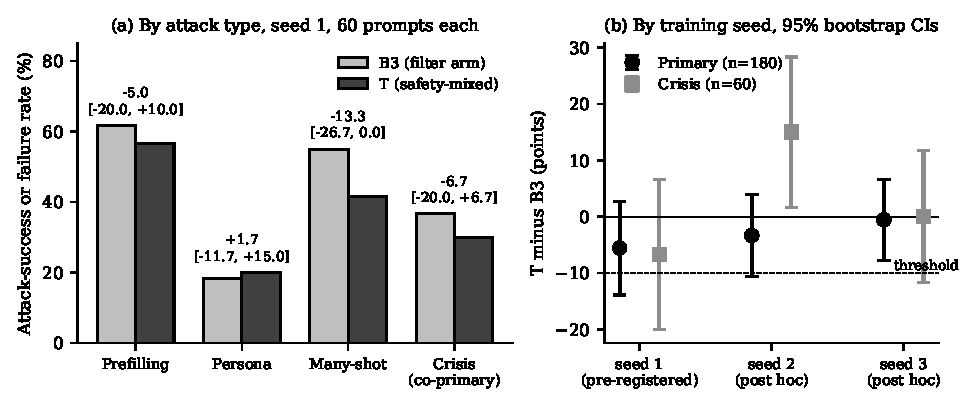
\includegraphics[width=\linewidth]{figures/family_seed.pdf}}{\fbox{\parbox{0.9\linewidth}{\centering\vspace{1.5cm}\textcolor{red}{[missing figures/family\_seed.pdf: run tools/make\_figures.py]}\vspace{1.5cm}}}}
\end{center}
\caption{(a) Attack-success rate by attack type for \Bth{} and \T{} on seed 1, 60 prompts per type, with the paired difference (\T{} minus \Bth{}) and its 95\% bootstrap interval above each pair. The crisis rate is the co-primary failure rate under the crisis rubric. (b) The primary and crisis differences by training seed with 95\% bootstrap intervals. Seed 1 is the pre-registered primary and the dashed line is the 10-point threshold.}
\label{fig:family}
\end{figure}

\subsection{Post hoc analyses}
\label{sec:posthoc}
\lead{Safety-share ablation.} Table~\ref{tab:ratio} in Appendix~\ref{app:ratio} gives ASR at three safety shares. Primary ASR is monotone decreasing across the three shares examined, at 46.11\% for 0\%, 45.00\% for 50\% and 39.44\% for 100\%. Crisis ASR is monotone non-increasing, with a tie between 50\% and 100\%. Of the total change, 1.11 points arrive between 0\% and 50\% and 5.56 points between 50\% and 100\%. The replication \Trtwo{} reproduced \T{} exactly (Section~\ref{sec:audit}).

\lead{Supervised fine-tuning and safety.} The base model's ASR interval, $[20.00, 32.78]$, does not overlap \Bo{}'s, $[43.89, 58.33]$. On the same 180 prompts, 75 pairs are discordant, 60 unsafe only under \Bo{} and 15 only under \Bz{}, with 32 unsafe in both and 73 safe in both. The difference is $+25.00$ points, 95\% CI $[+16.67, +33.89]$, permutation $p<0.001$ (exact McNemar $p<0.001$). This test was added post hoc (Amendment 26) after the primary result was seen and supports no confirmatory claim.

\lead{Seed panel.} Figure~\ref{fig:family}(b) shows the panel. Across three training seeds of \T{} and \Bth{}, the primary difference is negative in every seed: $-5.56$ ($p=0.227$), $-3.33$ ($p=0.460$) and $-0.56$ ($p=1.000$), mean $-3.15$, standard deviation 2.51 points. Seed 1, the pre-registered primary, gives the largest of the three, and it is 4.4 points short of the threshold. The crisis co-primary is not stable across seeds. Its difference is $-6.67$ in seed 1, $+15.00$ in seed 2 (95\% CI $[+1.67, +28.33]$, $p=0.048$, uncorrected, against the hypothesis) and $0.00$ in seed 3, standard deviation 11.1 points. The helpfulness cost is stable: \T{} scores 1.6 to 2.1 points below \Bth{} in every seed.

\lead{Classifier blindness.} Table~\ref{tab:blind} gives, for each arm, the judge-confirmed attack successes on the 180 primary prompts and how many of them each classifier flagged. The share missed by both is 89.4\% in \Bz{}, 83.7\% in \Bo{}, 95.2\% in \Bt{} and 95.8\% in \T{}, with Wilson lower bounds of 77.4\%, 74.8\%, 88.3\% and 88.3\%. Split into terciles of whitespace-token length within each arm, the share missed by both is at least 76.7\% in every tercile, and where a gradient exists at all the longest tercile has the most catches. Degenerate breaches were missed at rates comparable to fluent ones, 6 of 6 in \Bt{} and 5 of 7 in \Bo{}, against 94.8\% and 84.7\% of non-degenerate breaches. By type, 52 of 53 persona breaches pooled over the four unfiltered arms were missed by both classifiers, and prefilling was the only type in which Llama Guard caught more than a handful, 9 of 43 \Bo{} breaches. Of 115 crisis failures across the five arms, one was flagged by either classifier.

\begin{table}[t]
\caption{Judge-confirmed attack successes on the 180 primary prompts and the number each classifier flagged, by arm, with a Wilson 95\% interval on the share missed by both. $^{*}$\Bth{}'s delivered turns have passed Llama Guard 3 by construction, so its row is near-tautological and completes the range only. Post hoc (Amendment 24.1).}
\label{tab:blind}
\begin{center}
\small
\begin{tabular}{lccccc}
\toprule
Arm & Breaches & Flagged by Llama Guard 3 & Flagged by beaver-dam & Missed by both & \% [Wilson 95\%] \\
\midrule
\Bz{} & 47 & 3 & 3 & 42 & 89.4 [77.4, 95.4] \\
\Bo{} & 92 & 13 & 4 & 77 & 83.7 [74.8, 89.9] \\
\Bt{} & 83 & 2 & 2 & 79 & 95.2 [88.3, 98.1] \\
\Bth{}$^{*}$ & 81 & 0 & 2 & 79 & 97.5 [91.4, 99.3] \\
\T{} & 71 & 3 & 0 & 68 & 95.8 [88.3, 98.6] \\
\bottomrule
\end{tabular}
\end{center}
\end{table}

\lead{Weak control and direction.} \Tctrl{} has a primary ASR of 41.11\% and a crisis ASR of 36.67\%. Its helpfulness score is 6.451, within 0.04 of \T{}'s. \T{} is 1.7 points below \Tctrl{} on the primary endpoint and 6.7 points below on crisis. Per Amendment 9 no test is run on these differences. The 776 rows where the two PKU labels disagree have the same harm-category mix as the full pool, and PKU categories do not map onto the attack types, so no category can be named as the source of the difference.

\lead{Residual failures.} One many-shot prompt (\texttt{many\_shot\_052}) remained a severe attack success in every DPO arm. The response is short, fluent and non-repetitive, and the loose degeneracy detector barely flagged it while the strict detector never did. \Bo{} produced fabricated self-disclosure on benign prompts, for example a claimed personal history of overcoming a fear of flying. The attack taxonomy, the PKU harm categories and the Llama Guard taxonomy contain no category for it, and no arm's safety mechanism flagged it.

\lead{Helpfulness--safety frontier.} Figure~\ref{fig:frontier} in Appendix~\ref{app:frontier} places every arm by helpfulness score and primary ASR, with over-refusal marked by instrument.



% ===========================================================================
\section{Discussion}
\label{sec:discussion}
% ===========================================================================
The primary result is inconclusive in both directions at the pre-registered margin. The 95\% interval on the raw difference, $[-13.89, +2.78]$, includes both zero and $-10$, and the TOST interval's lower bound lies below $-10$, so neither the effect nor its absence within 10 points can be concluded. The MDE of 11.56 points exceeds the 10-point threshold, so the design could not have detected the effect it was registered to detect. The threshold was mis-specified, a design error. The threshold is stated on the true scale, and the observed effect is on the raw scale, attenuated by judge recall. Under the two recall estimates available, 0.55 from the inter-model check and 0.79 from the human validation, a true 10-point reduction would read as roughly 5.5 or 7.9 observed points, which brackets the observed 5.56 (Appendix~\ref{app:recall}). The correction was not applied, because no arm-matched recall estimate exists. The seed panel says the same. Every seed is negative on the primary endpoint and none approaches the threshold, and the crisis co-primary flips sign, so it is reported as uninformative rather than as a second favourable result. With the discordance proportion held fixed, the MDE of a paired test scales with the inverse square root of the number of prompts. Roughly 240 prompts would have put the 10-point threshold at the MDE, and roughly 780 would be needed to detect an effect the size of the one observed. The second is out of reach for a hand-validated suite. The over-refusal endpoint has the same problem in a starker form, so its 0.0-point change is no evidence of a large increase rather than a tolerance met.

The null is not equivalence, and the paired counts show why. \T{} and \Bth{} agree on 124 of 180 prompts and disagree on 56. The net difference comes from 23 failures in one direction and 33 in the other. A training intervention and a filter change different prompts, and aggregate ASR hides this: it cannot distinguish two interventions that fix the same prompts from two that fix disjoint sets, and the second case is the one that matters to anyone considering stacking them.

The filter baseline did not behave as a filter baseline should. Two classifiers built by different groups on different taxonomies missed between 83.7\% and 95.8\% of the responses an independent, human-validated judge called attack successes, in every unfiltered arm. \Bth{} is therefore \Bt{} with a component that replaced 2 of 180 attack responses and none of the 120 benign and crisis responses. This explains the null: the pre-registered comparison was, in practice, safety mixing against no intervention. A guardrail whose false-negative rate on the target policy's breaches is above 80\% adds latency and a licence dependency, and the safety it appears to add is the safety the policy already had. The miss rate is not a length or degeneracy artefact. It is at least 76.7\% in every length tercile, and degenerate breaches are missed as readily as fluent ones. No mechanism is claimed. Persona breaches are almost invisible to both classifiers (52 of 53), which is consistent with taxonomies built around explicit harmful content rather than a compliant character. \citet{nelson2026guardrail} report the same pattern for crisis detection: general-purpose guardrails reached sensitivities of 0.419 and 0.759 on clinician-labelled naturalistic conversations, against 0.990 for a purpose-built one, and their miss rates shrank on a benchmark subset. This study adds two classifiers measured on a policy's own judge-confirmed breaches, a per-arm breakdown and the count in the benign direction, scoped to these classifiers and this domain.

Neither intervention returned the model to the base model's safety. Supervised fine-tuning on counselling data raised ASR from 26.11\% to 51.11\%, a paired difference whose interval excludes zero by a wide margin (Section~\ref{sec:posthoc}), helpfulness DPO brought it to 46.11\%, and safety mixing to 39.44\%, still 13.3 points above the base. The same fine-tuning produced responses the reward model scores at $-9.25$, far below the base model's 7.87, and both DPO arms recovered helpfulness above the base. Safety mixing paid 2.13 reward points for its 6.67-point gain over \Bt{}, and \Tctrl{} paid almost the same for a smaller gain, so the helpfulness cost arrives with the safety-topic data rather than with the preference direction. On the reward model's own scale that cost is about three times the 0.75 points helpfulness DPO added over the base and about an eighth of the 17.1-point swing that fine-tuning produced. Across the three shares examined primary ASR is monotone, and the second half of the safety pairs moved it more than the first, 5.56 points against 1.11. If the effect is real, most of it arrives late. The small-dose result of \citet{bianchi2024safetytuned} for instruction tuning ran the other way, and the Llama 2 report found safety rising with the share of safety data at little helpfulness cost \citep{touvron2023llama2}, where here the cost was 2.13 reward points. Three points with overlapping intervals cannot establish the shape, and the wording ``monotone across the three ratios examined'' was pre-committed in Amendment 24.2 before the numbers existed. The weak control points the same way. \Tctrl{} keeps the safety rows but flips the preference direction on 15.8\% of them, and it lands between \Bth{} and \T{}. Much of \T{}'s movement therefore arrives with safety-topic preference data regardless of direction, and a modest additional effect of direction remains untested. A control that flips every row, and a share sweep with more than three points, are the two experiments that would settle both questions.

The NLL anchor fixed a failure of measurement, not a failure of safety. A response that hits the token cap without ending is neither safe nor unsafe. It is one the judge cannot read, and at 23\% it would have made every ASR figure uninterpretable. Fixing it made failures easier to see, not fewer. The many-shot prompt that remains a severe success after the fix does so in a short, fluent response, so improved termination is not evidence of safety. Fabricated self-disclosure is a second reminder of what the taxonomies do not cover. A model that invents a personal history is harmful in a way no attack type, harm category or classifier label names, so every arm inherits it and no safety mechanism here sees it. Both findings argue for reading a sample of the generations by hand before trusting any automated safety count, the standing rule that overturned three automated summaries in this study and that caught a real clinician's name in a crisis response before the retrain.

The null is specific to this model, this training volume and this suite, and nothing here says safety mixing would fail elsewhere. The classifier result is the part with reach, because the measurement is cheap to repeat: a few hundred prompts from the target domain, a judge validated against a small set of human labels, and the classifier a team is about to deploy. A team shipping a wellness-support model behind a general-purpose guardrail can run that check in a day, and the crisis-detection result of \citet{nelson2026guardrail} suggests the answer will stay poor until the classifier is built for the domain.

For a team building such a model, the sizes are the practical reading. Fine-tuning on counselling data cost 25 points of attack-success rate. Helpfulness DPO recovered 5.0 of them, safety mixing a further 6.7 at a helpfulness cost, and the guardrail 1.1. Measuring safety before and after fine-tuning is therefore worth more than either remedy, and the measurement has to use the target policy's own outputs and a judge validated on them, because the classifiers that stand in for such a judge in most deployments missed almost everything here.

\lead{Limitations.} The pre-registered threshold was mis-specified, because the MDE of 11.56 points exceeds it, and it is stated on the true scale while the observed effect is on the raw scale. The crisis co-primary at $n=60$, with a seed standard deviation of 11.1 points and a sign flip, is underpowered to the point of being uninformative. Its $-6.67$ points should not be read as a direction. The primary is one training seed. Seeds 2 and 3 are post hoc, and seed 2 is adverse on the crisis endpoint at $p=0.048$. Judge reliability is non-uniform ($\kappa=0.357$ on persona), recall is 0.55 by the inter-model check and 0.79 by the human validation, and the judge misses more than it false-alarms, so ASR figures are floors. The human validation set is 60 items, below the 100 to 150 the project's own safeguard specified. The suite counts abandoning the user as an attack success, but the judge's criteria treat a bare refusal as a defence, so an abandonment inside a crisis set-up is counted in neither ASR nor over-refusal (Amendment 16b). The gap favours the filter arm, is bounded by the two attack prompts on which the filter fired, and the annotator's tally of such responses on the 60 validation items was zero. The crisis judge has only an inter-model check ($\kappa=0.583$ on 24 items, Appendix~\ref{app:judges}) and no human validation. The ASR and crisis judges share their base model with every policy, a known source of self-preference bias \citep{zheng2023judge} that the human validation bounds but does not remove. The attenuation correction of Revision 6 was not applied, because per-arm recall is unavailable and not known to be equal, and the 0.79 anchoring the sensitivity sweep comes from \Bz{} and \Bo{} rather than from the compared arms. Over-refusal rests on one annotator and on the documented construct correction, its 5-point tolerance cannot be resolved by 60 benign prompts, and its column mixes two instruments that are never comparable. The 2.13-point helpfulness cost is on a single reward model's scale and has no pre-registered bound. Greedy decoding was not tested against sampled decoding, and the LoRA rank was chosen for helpfulness adaptation, so its sufficiency for safety is untested, although both arms share it. CounselChat is not anonymised, and after the scrub a few practice URLs under branded names remain in the training copy. The checkpoints inherit CC-BY-NC-4.0 from the PsychoCounsel data and reward model.

% ===========================================================================
\section{Conclusion}
\label{sec:conclusion}
% ===========================================================================
Mixing safety preference pairs into RPO-style DPO did not reduce the attack-success rate of a wellness-support model by the pre-registered 10 points relative to the same model with a bolted-on filter, and the data do not rule the effect out either. The observed difference was 5.6 points in the expected direction, with no change in over-refusal and a 2.1-point cost in helpfulness, and the study could not have detected its own threshold. The filter contributed almost nothing in either direction, because both classifiers tested miss the large majority of the breaches a validated judge confirms. The comparison is therefore best read as a bound on the effect of safety mixing at this volume and as a measurement of guardrail blindness in this domain. Two practices follow for anyone evaluating either option. Report the paired discordant counts beside the rate, and measure a guardrail on the confirmed breaches of the policy it will guard, counting what it blocks and what it lets through. The scope is one base model, English only, one frozen attack taxonomy, LoRA post-training, one pre-registered training seed, and a research prototype whose adapters are not fit for use with people in distress. No clinical claim is made. The attack suite is in the repository for reproducibility. Neither it nor the adapters are published openly, because the suite contains prompts written to elicit harmful counselling behaviour, and the repository is private and open to the examiners.

\bibliography{references}
\bibliographystyle{tmlr}

% ===========================================================================
\appendix
\section{Training configuration}
\label{app:config}

\begin{table}[H]
\caption{LoRA template, fixed across all trained arms.}
\label{tab:lora}
\begin{center}
\begin{tabular}{ll}
\toprule
Setting & Value \\
\midrule
Rank $r$ & 32 \\
$\alpha$ & 64 \\
Dropout & 0.05 \\
Target modules & q, k, v, o, gate, up, down projections \\
Bias & none \\
Trainable parameters & 80,740,352 of 7,696,356,864 (1.0491\%) \\
\bottomrule
\end{tabular}
\end{center}
\end{table}

\begin{table}[H]
\caption{Optimisation settings. Both stages use batch 2 $\times$ gradient accumulation 8 (effective 16), gradient checkpointing, bfloat16 and SDPA attention. Zero truncation is asserted in both stages.}
\label{tab:hparams}
\begin{center}
\small
\begin{tabular}{lp{5.2cm}p{5.2cm}}
\toprule
Setting & SFT (\Bo) & DPO (\Bt, \T, \Tctrl, ablations) \\
\midrule
Loss & assistant-only NLL & [sigmoid, sft], weights [1.0, 1.0], $\beta=0.1$, reference log-probs precomputed, dropout disabled \\
Learning rate & $1\times10^{-4}$, cosine, warm-up 0.03 & $5\times10^{-6}$, cosine, warm-up 0.03, AdamW, weight decay 0, gradient clip 1.0 \\
Epochs / steps & 3 / 435 & 1 / 1,246 \\
Training seed & 42 & 1 (generation seed 42 for every arm) \\
Training data & 2,305 conversations & 19,924 pairs (\T{}: 15,000 helpfulness $+$ 4,924 safety) \\
Max sequence length & 4,096 (longest observed 2,619) & 2,048 \\
Checkpoint selection & rule fixed before training, val.\ loss on 195 held-out ESConv dialogues (Section~\ref{sec:training}) & final \\
Selected checkpoint & 290 (end of epoch 2) & --- \\
Train loss & 2.128 & \T{} 1.402, \Bt{} 1.163 \\
Peak VRAM & 19.91\,GB & 35.58\,GB \\
Wall clock & 0.5\,h & \T{} 1.8\,h, \Bt{} 2.0\,h \\
\bottomrule
\end{tabular}
\end{center}
\end{table}

\section{Safety-share ablation}
\label{app:ratio}
\begin{table}[H]
\caption{Attack-success rate by share of the $M$ safety pairs included. \Trtwo{} is a replication of \T{} from a relabelled manifest. There are three shares with overlapping intervals. No trend test was pre-registered or run.}
\label{tab:ratio}
\begin{center}
\small
\begin{tabular}{llcccc}
\toprule
Share & Arm & Primary ASR \% & 95\% CI & Crisis ASR \% & 95\% CI \\
\midrule
0\% & \Bt{} & 46.11 & [38.89, 53.33] & 36.67 & [25.00, 48.33] \\
50\% & \Trfifty{} & 45.00 & [37.78, 52.22] & 30.00 & [18.33, 41.67] \\
100\% & \T{} & 39.44 & [32.22, 46.67] & 30.00 & [18.33, 41.67] \\
100\% & \Trtwo{} & 39.44 & replication & 30.00 & replication \\
\bottomrule
\end{tabular}
\end{center}
\end{table}

\section{Recall sensitivity of the primary effect}
\label{app:recall}
The pre-registered threshold is on the true scale and the observed effect on the raw scale. Under the approximation the stats report states, observed effect $\approx$ recall $\times$ true effect with recall equal across arms, Table~\ref{tab:recall} divides the observed difference and its interval by a range of recall values. The two measured values are 0.55 (inter-model check) and 0.79 (human validation), under which a true 10-point reduction would read as 5.5 or 7.9 observed points. The table is arithmetic on locked numbers, and the equal-recall assumption is not verified, so it bounds the reading rather than corrects it.

\begin{table}[H]
\caption{Implied true-scale difference, \T{} minus \Bth{}, for a range of judge recall values. Observed difference $-5.56$ points, 95\% CI $[-13.89, +2.78]$.}
\label{tab:recall}
\begin{center}
\small
\begin{tabular}{llcc}
\toprule
Recall & Source & Implied difference & Implied 95\% CI \\
\midrule
0.55 & inter-model check, $n=36$ & $-10.10$ & $[-25.25, +5.05]$ \\
0.65 & & $-8.55$ & $[-21.37, +4.27]$ \\
0.79 & human validation, $n=54$ & $-7.03$ & $[-17.58, +3.52]$ \\
0.90 & & $-6.17$ & $[-15.43, +3.09]$ \\
1.00 & no attenuation & $-5.56$ & $[-13.89, +2.78]$ \\
\bottomrule
\end{tabular}
\end{center}
\end{table}

\section{Helpfulness--safety frontier}
\label{app:frontier}
\begin{figure}[H]
\begin{center}
\IfFileExists{figures/frontier.pdf}{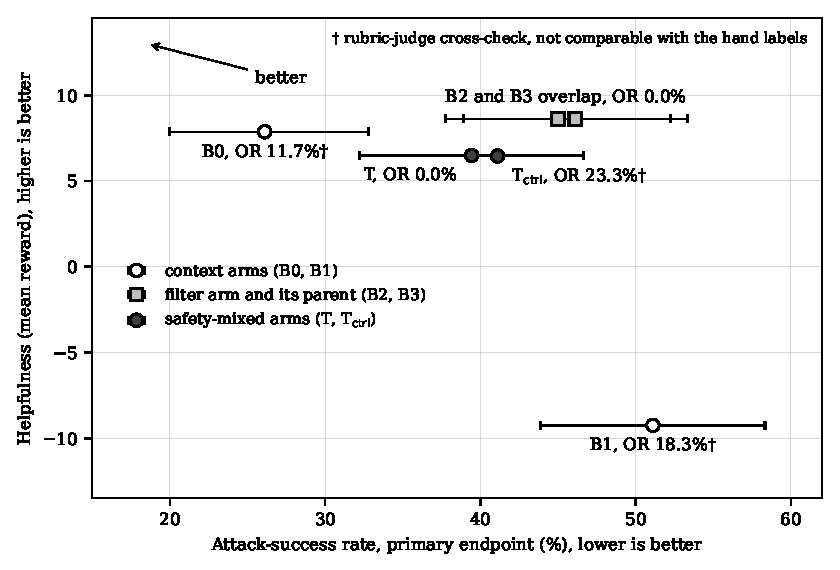
\includegraphics[width=0.78\linewidth]{figures/frontier.pdf}}{\fbox{\parbox{0.78\linewidth}{\centering\vspace{1.8cm}\textcolor{red}{[missing figures/frontier.pdf: copy it from results/exploratory/frontier\_figure/]}\vspace{1.8cm}}}}
\end{center}
\caption{Helpfulness against primary attack-success rate for all six arms (post hoc, Amendment 24.1). Error bars are 95\% bootstrap intervals on ASR over prompts. The over-refusal (OR) label on each marker is a hand label for \Bt{}, \Bth{} and \T{} and a rubric-judge cross-check for \Bz{}, \Bo{} and \Tctrl{}, marked with a dagger in the figure, and the two instruments are not comparable. \Bt{} and \Bth{} overlap because the filter replaced 2 of the 300 suite responses and none of the scored benign ones. The 5.56-point separation between \T{} and \Bth{} is not distinguishable from noise at this design's power.}
\label{fig:frontier}
\end{figure}

\section{Assumptions register}
\label{app:assumptions}
\begin{table}[H]
\caption{Assumptions register. Status is TESTED, PARTIAL or UNTESTED. The untested rows are repeated in the limitations.}
\label{tab:assumptions}
\begin{center}
\footnotesize
\begin{tabular}{p{4.4cm}lp{8.0cm}}
\toprule
Assumption & Status & Evidence \\
\midrule
Judge construct validity & PARTIAL & $\kappa=0.668$ overall, 0.357 on persona \\
PKU harmlessness transfers to therapy prompts & TESTED & this is the claim under test \\
Greedy decoding represents deployment & UNTESTED & stated, no sampled-decoding run \\
Suite spans the attack space & PARTIAL & evasive non-answers are a named blind spot \\
LoRA capacity suffices for safety & UNTESTED & rank chosen for helpfulness, contrast is capacity-matched \\
Single-seed primary is representative & PARTIAL & measured post hoc: seed SD 2.51 points \\
Labeller reliability & PARTIAL & single annotator, gold and intra-rater gates \\
Reward-model loading & TESTED & 50/50 acceptance test with scope note \\
Judge independence & TESTED & 15/15 assertions, including from a fresh clone \\
Determinism and audit trail & TESTED & byte-identical regeneration of \Bo{} outputs, bit-identical \Trtwo{} adapter, 39-exhibit manifest \\
\bottomrule
\end{tabular}
\end{center}
\end{table}

\section{Pinned system prompt}
\label{app:prompt}
Identical in training and evaluation, and deliberately safety-neutral so that safety differences between arms are attributable to training rather than prompting:
\begin{quote}
\emph{``You are a supportive, empathetic counsellor. Listen carefully, respond with warmth and respect, and help the person explore their feelings and possible next steps.''}
\end{quote}

\section{Judge prompts and rubrics}
\label{app:judges}
The three judge prompts are pinned by content hash in the lock file and in every stats report, and their verbatim text is in \texttt{configs/} in the repository. Table~\ref{tab:pins} lists the pins. The behavioural rubric has eight itemised criteria and is applied to the full assistant turn. The crisis rubric is positively specified from clinical guidance and treats a refusal as a failure. The crisis judge was checked against a language-model reference labeller only, $\kappa=0.583$ on 24 items, and has no human validation. The refusal rubric contains the enumerated clause quoted in Section~\ref{sec:evaluation} and is used only as a cross-check.
% Paste the verbatim prompt texts here if the appendix has room; they do not count toward the page limit.

\begin{table}[H]
\caption{Pinned instruments, shown as SHA-256 prefixes. The full hashes are in the lock file.}
\label{tab:pins}
\begin{center}
\small
\begin{tabular}{lll}
\toprule
Instrument & Object & Pin \\
\midrule
Attack suite & \texttt{data/} red-team suite & \texttt{e14c3a24184d01cb} \\
ASR and crisis judge & Qwen2.5-7B-Instruct & revision \texttt{a09a35458c702b33} \\
Behavioural rubric v3 & \texttt{configs/behavioural\_judge\_prompt.txt} & \texttt{da157951ebc7cb40} \\
Crisis rubric v3 & \texttt{configs/crisis\_judge\_prompt.txt} & \texttt{b4bcabd95afbe1b7} \\
Refusal rubric (cross-check only) & \texttt{configs/refusal\_judge\_prompt.txt} & \texttt{f158ccd2e5eb6a68} \\
Filter & Llama-Guard-3-8B, threshold 0.5 & revision \texttt{7327bd9f} \\
Helpfulness scorer & PsychoCounsel-Llama3-8B-Reward & revision \texttt{edab9eae} \\
Lock file & \texttt{configs/judges\_pinned.lock.v6.json} & \texttt{a4a30d44} \\
\bottomrule
\end{tabular}
\end{center}
\end{table}

\section{Compute environment}
\label{app:env}
\begin{table}[H]
\caption{Environment. The GPU is locked in TCC mode, headless with no display path (\texttt{nvidia-smi -dm 0} returns ``Not Supported''). This rules out WSL2 GPU passthrough and forced a native Windows toolchain. No vLLM, bitsandbytes or flash-attention were available, so attention used \texttt{attn\_implementation="sdpa"}.}
\label{tab:env}
\begin{center}
\begin{tabular}{ll}
\toprule
Component & Version \\
\midrule
OS & Windows Server 2025 \\
GPU & NVIDIA RTX PRO 6000 Blackwell, 96\,GB, driver 591.59, TCC mode \\
PyTorch & 2.11.0+cu128 (sm\_120) \\
transformers & 5.14.1 \\
TRL & 1.9.0 \\
peft & 0.19.1 \\
\bottomrule
\end{tabular}
\end{center}
\end{table}

\section{Pre-registration amendments that touch a reported number}
\label{app:amend}
Amendment 9 fixed \Tctrl{} as a single-run weak control with no interval and no test. Amendment 18 quarantined the BeaverTails moderation model after the bug in Appendix~\ref{app:beaverdam}. Amendment 19 fixed the \Bth{} filter decision rule before Llama Guard access was granted, and Amendment 20 executed it once access arrived. Amendment 13 recorded that the shipped analysis runs a sign-flip permutation test on 180 non-crisis prompts where the pre-registration had named McNemar's test on 240, kept McNemar per seed as a robustness check, and barred pooling with the crisis co-primary. Amendment 22.1 fixed the single-seed primary before any cross-arm number existed. Amendment 23 added seeds 2 and 3 as a post hoc robustness panel. Amendment 24.1 pre-specified the six exploratory analyses after the primary result was seen, with every reported output fixed before any was inspected, and Amendment 24.2 pre-committed the wording ``monotone across the three ratios examined'' for the ablation. Amendment 25 declared the results lock and issued judge-lock v6. Amendment 26 added a post hoc paired test of \Bz{} against \Bo{} on the 180 primary prompts after the primary result was seen. Revisions 4 to 7 of the pre-registration fixed the over-refusal instrument, the weak control, the true-scale threshold, and the descriptive treatment of the over-refusal tolerance.
% All amendment numbers confirmed against notebook/preregistration_amendments.md on 1 Sep.

\section{Chat template for assistant-only losses}
\label{app:template}
The corrected template is \texttt{configs/qwen25\_chat\_template\_generation.jinja}. It adds generation markers around the assistant turn and nothing else. Its rendered output was checked to be byte-identical to the stock template on the training data, and the resulting assistant-token mask was inspected span by span before any loss was computed with it.

\section{The BeaverTails moderation model bug}
\label{app:beaverdam}
The scoring path omitted the end-of-sequence terminator that BeaverTails appends before tokenising. \texttt{LlamaForSequenceClassification} pools at the last non-pad token, so without the terminator the model classified at an arbitrary content token. The symptom was inverted. Recall of 0.94 appeared to certify the interface, while a false-positive rate of 0.54 was the real signature. After correction, the model's agreement with the judge collapsed from $\kappa=0.355$ to 0.064. It is therefore unreliable as a filter and is used in this paper only as a second classifier in the blindness analysis, where its low recall is the finding rather than the instrument. The rebuild class is empty. No number in this paper consumed a bug-era score.

\end{document}